% Created by tikzDevice version 0.12.3.1 on 2023-04-24 17:26:44
% !TEX encoding = UTF-8 Unicode
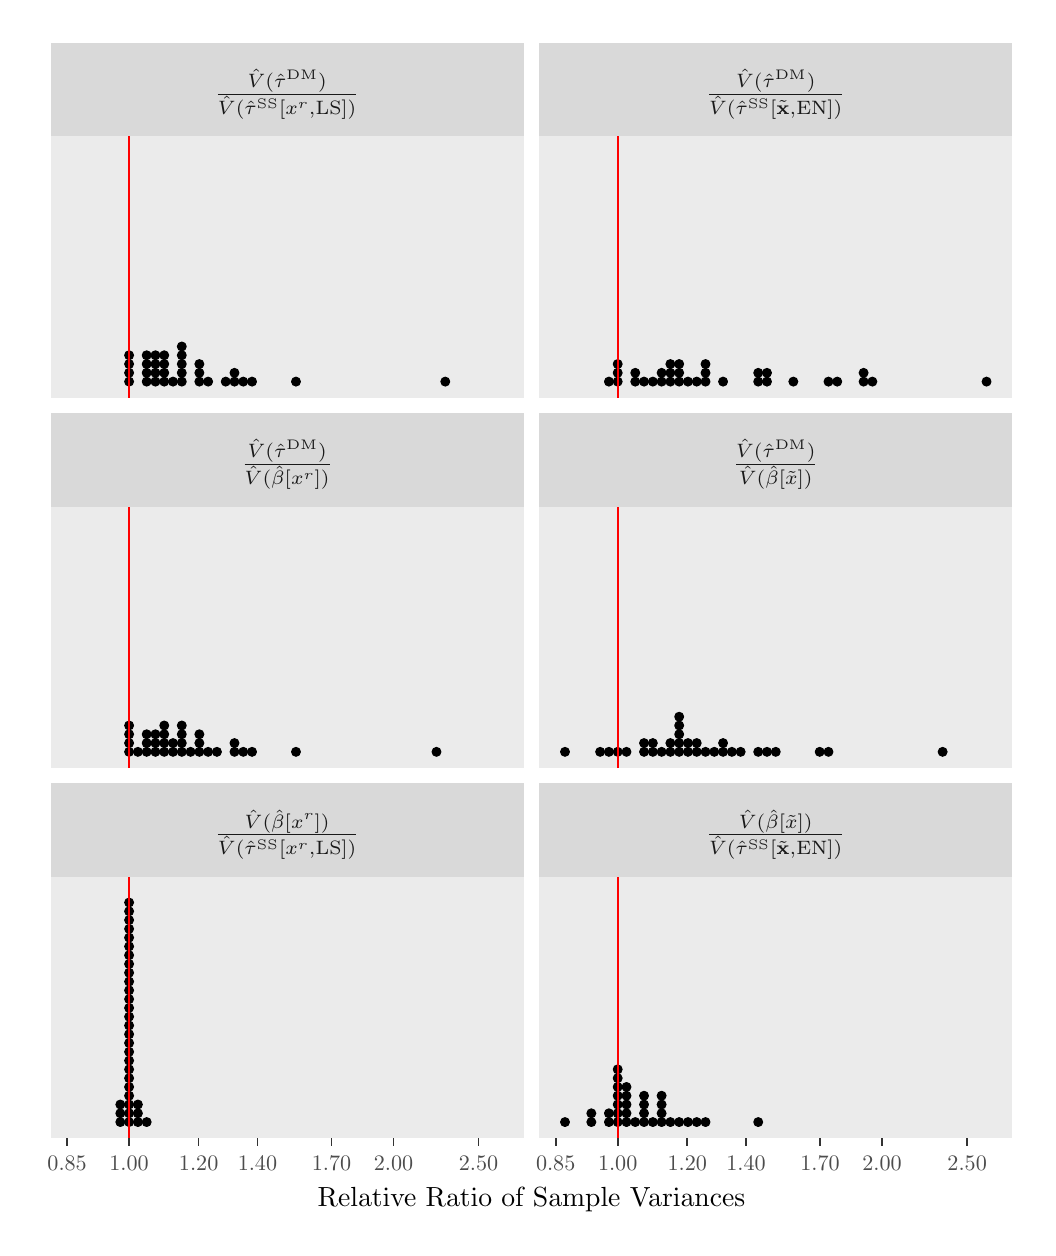
\begin{tikzpicture}[x=1pt,y=1pt]
\definecolor{fillColor}{RGB}{255,255,255}
\path[use as bounding box,fill=fillColor,fill opacity=0.00] (0,0) rectangle (361.35,433.62);
\begin{scope}
\path[clip] (  0.00,  0.00) rectangle (361.35,433.62);
\definecolor{drawColor}{RGB}{255,255,255}
\definecolor{fillColor}{RGB}{255,255,255}

\path[draw=drawColor,line width= 0.6pt,line join=round,line cap=round,fill=fillColor] (  0.00,  0.00) rectangle (361.35,433.62);
\end{scope}
\begin{scope}
\path[clip] (  8.25,299.84) rectangle (179.30,394.32);
\definecolor{fillColor}{gray}{0.92}

\path[fill=fillColor] (  8.25,299.84) rectangle (179.30,394.32);
\definecolor{drawColor}{RGB}{0,0,0}
\definecolor{fillColor}{RGB}{0,0,0}

\path[draw=drawColor,line width= 0.4pt,line join=round,fill=fillColor] ( 36.65,305.72) circle (  1.59);

\path[draw=drawColor,line width= 0.4pt,line join=round,fill=fillColor] ( 36.65,308.89) circle (  1.59);

\path[draw=drawColor,line width= 0.4pt,line join=round,fill=fillColor] ( 36.65,312.07) circle (  1.59);

\path[draw=drawColor,line width= 0.4pt,line join=round,fill=fillColor] ( 36.65,315.24) circle (  1.59);

\path[draw=drawColor,line width= 0.4pt,line join=round,fill=fillColor] ( 43.00,305.72) circle (  1.59);

\path[draw=drawColor,line width= 0.4pt,line join=round,fill=fillColor] ( 43.00,308.89) circle (  1.59);

\path[draw=drawColor,line width= 0.4pt,line join=round,fill=fillColor] ( 43.00,312.07) circle (  1.59);

\path[draw=drawColor,line width= 0.4pt,line join=round,fill=fillColor] ( 43.00,315.24) circle (  1.59);

\path[draw=drawColor,line width= 0.4pt,line join=round,fill=fillColor] ( 46.17,305.72) circle (  1.59);

\path[draw=drawColor,line width= 0.4pt,line join=round,fill=fillColor] ( 46.17,308.89) circle (  1.59);

\path[draw=drawColor,line width= 0.4pt,line join=round,fill=fillColor] ( 46.17,312.07) circle (  1.59);

\path[draw=drawColor,line width= 0.4pt,line join=round,fill=fillColor] ( 46.17,315.24) circle (  1.59);

\path[draw=drawColor,line width= 0.4pt,line join=round,fill=fillColor] ( 49.35,305.72) circle (  1.59);

\path[draw=drawColor,line width= 0.4pt,line join=round,fill=fillColor] ( 49.35,308.89) circle (  1.59);

\path[draw=drawColor,line width= 0.4pt,line join=round,fill=fillColor] ( 49.35,312.07) circle (  1.59);

\path[draw=drawColor,line width= 0.4pt,line join=round,fill=fillColor] ( 49.35,315.24) circle (  1.59);

\path[draw=drawColor,line width= 0.4pt,line join=round,fill=fillColor] ( 52.52,305.72) circle (  1.59);

\path[draw=drawColor,line width= 0.4pt,line join=round,fill=fillColor] ( 55.69,305.72) circle (  1.59);

\path[draw=drawColor,line width= 0.4pt,line join=round,fill=fillColor] ( 55.69,308.89) circle (  1.59);

\path[draw=drawColor,line width= 0.4pt,line join=round,fill=fillColor] ( 55.69,312.07) circle (  1.59);

\path[draw=drawColor,line width= 0.4pt,line join=round,fill=fillColor] ( 55.69,315.24) circle (  1.59);

\path[draw=drawColor,line width= 0.4pt,line join=round,fill=fillColor] ( 55.69,318.41) circle (  1.59);

\path[draw=drawColor,line width= 0.4pt,line join=round,fill=fillColor] ( 62.04,305.72) circle (  1.59);

\path[draw=drawColor,line width= 0.4pt,line join=round,fill=fillColor] ( 62.04,308.89) circle (  1.59);

\path[draw=drawColor,line width= 0.4pt,line join=round,fill=fillColor] ( 62.04,312.07) circle (  1.59);

\path[draw=drawColor,line width= 0.4pt,line join=round,fill=fillColor] ( 65.21,305.72) circle (  1.59);

\path[draw=drawColor,line width= 0.4pt,line join=round,fill=fillColor] ( 71.56,305.72) circle (  1.59);

\path[draw=drawColor,line width= 0.4pt,line join=round,fill=fillColor] ( 74.73,305.72) circle (  1.59);

\path[draw=drawColor,line width= 0.4pt,line join=round,fill=fillColor] ( 74.73,308.89) circle (  1.59);

\path[draw=drawColor,line width= 0.4pt,line join=round,fill=fillColor] ( 77.91,305.72) circle (  1.59);

\path[draw=drawColor,line width= 0.4pt,line join=round,fill=fillColor] ( 81.08,305.72) circle (  1.59);

\path[draw=drawColor,line width= 0.4pt,line join=round,fill=fillColor] ( 96.95,305.72) circle (  1.59);

\path[draw=drawColor,line width= 0.4pt,line join=round,fill=fillColor] (150.90,305.72) circle (  1.59);
\definecolor{drawColor}{RGB}{255,0,0}

\path[draw=drawColor,line width= 0.6pt,line join=round] ( 36.65,299.84) -- ( 36.65,394.32);
\end{scope}
\begin{scope}
\path[clip] (  8.25,166.06) rectangle (179.30,260.54);
\definecolor{fillColor}{gray}{0.92}

\path[fill=fillColor] (  8.25,166.06) rectangle (179.30,260.54);
\definecolor{drawColor}{RGB}{0,0,0}
\definecolor{fillColor}{RGB}{0,0,0}

\path[draw=drawColor,line width= 0.4pt,line join=round,fill=fillColor] ( 36.65,171.94) circle (  1.59);

\path[draw=drawColor,line width= 0.4pt,line join=round,fill=fillColor] ( 36.65,175.11) circle (  1.59);

\path[draw=drawColor,line width= 0.4pt,line join=round,fill=fillColor] ( 36.65,178.29) circle (  1.59);

\path[draw=drawColor,line width= 0.4pt,line join=round,fill=fillColor] ( 36.65,181.46) circle (  1.59);

\path[draw=drawColor,line width= 0.4pt,line join=round,fill=fillColor] ( 39.83,171.94) circle (  1.59);

\path[draw=drawColor,line width= 0.4pt,line join=round,fill=fillColor] ( 43.00,171.94) circle (  1.59);

\path[draw=drawColor,line width= 0.4pt,line join=round,fill=fillColor] ( 43.00,175.11) circle (  1.59);

\path[draw=drawColor,line width= 0.4pt,line join=round,fill=fillColor] ( 43.00,178.29) circle (  1.59);

\path[draw=drawColor,line width= 0.4pt,line join=round,fill=fillColor] ( 46.17,171.94) circle (  1.59);

\path[draw=drawColor,line width= 0.4pt,line join=round,fill=fillColor] ( 46.17,175.11) circle (  1.59);

\path[draw=drawColor,line width= 0.4pt,line join=round,fill=fillColor] ( 46.17,178.29) circle (  1.59);

\path[draw=drawColor,line width= 0.4pt,line join=round,fill=fillColor] ( 49.35,171.94) circle (  1.59);

\path[draw=drawColor,line width= 0.4pt,line join=round,fill=fillColor] ( 49.35,175.11) circle (  1.59);

\path[draw=drawColor,line width= 0.4pt,line join=round,fill=fillColor] ( 49.35,178.29) circle (  1.59);

\path[draw=drawColor,line width= 0.4pt,line join=round,fill=fillColor] ( 49.35,181.46) circle (  1.59);

\path[draw=drawColor,line width= 0.4pt,line join=round,fill=fillColor] ( 52.52,171.94) circle (  1.59);

\path[draw=drawColor,line width= 0.4pt,line join=round,fill=fillColor] ( 52.52,175.11) circle (  1.59);

\path[draw=drawColor,line width= 0.4pt,line join=round,fill=fillColor] ( 55.69,171.94) circle (  1.59);

\path[draw=drawColor,line width= 0.4pt,line join=round,fill=fillColor] ( 55.69,175.11) circle (  1.59);

\path[draw=drawColor,line width= 0.4pt,line join=round,fill=fillColor] ( 55.69,178.29) circle (  1.59);

\path[draw=drawColor,line width= 0.4pt,line join=round,fill=fillColor] ( 55.69,181.46) circle (  1.59);

\path[draw=drawColor,line width= 0.4pt,line join=round,fill=fillColor] ( 58.87,171.94) circle (  1.59);

\path[draw=drawColor,line width= 0.4pt,line join=round,fill=fillColor] ( 62.04,171.94) circle (  1.59);

\path[draw=drawColor,line width= 0.4pt,line join=round,fill=fillColor] ( 62.04,175.11) circle (  1.59);

\path[draw=drawColor,line width= 0.4pt,line join=round,fill=fillColor] ( 62.04,178.29) circle (  1.59);

\path[draw=drawColor,line width= 0.4pt,line join=round,fill=fillColor] ( 65.21,171.94) circle (  1.59);

\path[draw=drawColor,line width= 0.4pt,line join=round,fill=fillColor] ( 68.39,171.94) circle (  1.59);

\path[draw=drawColor,line width= 0.4pt,line join=round,fill=fillColor] ( 74.73,171.94) circle (  1.59);

\path[draw=drawColor,line width= 0.4pt,line join=round,fill=fillColor] ( 74.73,175.11) circle (  1.59);

\path[draw=drawColor,line width= 0.4pt,line join=round,fill=fillColor] ( 77.91,171.94) circle (  1.59);

\path[draw=drawColor,line width= 0.4pt,line join=round,fill=fillColor] ( 81.08,171.94) circle (  1.59);

\path[draw=drawColor,line width= 0.4pt,line join=round,fill=fillColor] ( 96.95,171.94) circle (  1.59);

\path[draw=drawColor,line width= 0.4pt,line join=round,fill=fillColor] (147.72,171.94) circle (  1.59);
\definecolor{drawColor}{RGB}{255,0,0}

\path[draw=drawColor,line width= 0.6pt,line join=round] ( 36.65,166.06) -- ( 36.65,260.54);
\end{scope}
\begin{scope}
\path[clip] (  8.25, 32.28) rectangle (179.30,126.76);
\definecolor{fillColor}{gray}{0.92}

\path[fill=fillColor] (  8.25, 32.28) rectangle (179.30,126.76);
\definecolor{drawColor}{RGB}{0,0,0}
\definecolor{fillColor}{RGB}{0,0,0}

\path[draw=drawColor,line width= 0.4pt,line join=round,fill=fillColor] ( 33.48, 38.16) circle (  1.59);

\path[draw=drawColor,line width= 0.4pt,line join=round,fill=fillColor] ( 33.48, 41.33) circle (  1.59);

\path[draw=drawColor,line width= 0.4pt,line join=round,fill=fillColor] ( 33.48, 44.50) circle (  1.59);

\path[draw=drawColor,line width= 0.4pt,line join=round,fill=fillColor] ( 36.65, 38.16) circle (  1.59);

\path[draw=drawColor,line width= 0.4pt,line join=round,fill=fillColor] ( 36.65, 41.33) circle (  1.59);

\path[draw=drawColor,line width= 0.4pt,line join=round,fill=fillColor] ( 36.65, 44.50) circle (  1.59);

\path[draw=drawColor,line width= 0.4pt,line join=round,fill=fillColor] ( 36.65, 47.68) circle (  1.59);

\path[draw=drawColor,line width= 0.4pt,line join=round,fill=fillColor] ( 36.65, 50.85) circle (  1.59);

\path[draw=drawColor,line width= 0.4pt,line join=round,fill=fillColor] ( 36.65, 54.02) circle (  1.59);

\path[draw=drawColor,line width= 0.4pt,line join=round,fill=fillColor] ( 36.65, 57.20) circle (  1.59);

\path[draw=drawColor,line width= 0.4pt,line join=round,fill=fillColor] ( 36.65, 60.37) circle (  1.59);

\path[draw=drawColor,line width= 0.4pt,line join=round,fill=fillColor] ( 36.65, 63.54) circle (  1.59);

\path[draw=drawColor,line width= 0.4pt,line join=round,fill=fillColor] ( 36.65, 66.72) circle (  1.59);

\path[draw=drawColor,line width= 0.4pt,line join=round,fill=fillColor] ( 36.65, 69.89) circle (  1.59);

\path[draw=drawColor,line width= 0.4pt,line join=round,fill=fillColor] ( 36.65, 73.06) circle (  1.59);

\path[draw=drawColor,line width= 0.4pt,line join=round,fill=fillColor] ( 36.65, 76.24) circle (  1.59);

\path[draw=drawColor,line width= 0.4pt,line join=round,fill=fillColor] ( 36.65, 79.41) circle (  1.59);

\path[draw=drawColor,line width= 0.4pt,line join=round,fill=fillColor] ( 36.65, 82.59) circle (  1.59);

\path[draw=drawColor,line width= 0.4pt,line join=round,fill=fillColor] ( 36.65, 85.76) circle (  1.59);

\path[draw=drawColor,line width= 0.4pt,line join=round,fill=fillColor] ( 36.65, 88.93) circle (  1.59);

\path[draw=drawColor,line width= 0.4pt,line join=round,fill=fillColor] ( 36.65, 92.11) circle (  1.59);

\path[draw=drawColor,line width= 0.4pt,line join=round,fill=fillColor] ( 36.65, 95.28) circle (  1.59);

\path[draw=drawColor,line width= 0.4pt,line join=round,fill=fillColor] ( 36.65, 98.45) circle (  1.59);

\path[draw=drawColor,line width= 0.4pt,line join=round,fill=fillColor] ( 36.65,101.63) circle (  1.59);

\path[draw=drawColor,line width= 0.4pt,line join=round,fill=fillColor] ( 36.65,104.80) circle (  1.59);

\path[draw=drawColor,line width= 0.4pt,line join=round,fill=fillColor] ( 36.65,107.97) circle (  1.59);

\path[draw=drawColor,line width= 0.4pt,line join=round,fill=fillColor] ( 36.65,111.15) circle (  1.59);

\path[draw=drawColor,line width= 0.4pt,line join=round,fill=fillColor] ( 36.65,114.32) circle (  1.59);

\path[draw=drawColor,line width= 0.4pt,line join=round,fill=fillColor] ( 36.65,117.49) circle (  1.59);

\path[draw=drawColor,line width= 0.4pt,line join=round,fill=fillColor] ( 39.83, 38.16) circle (  1.59);

\path[draw=drawColor,line width= 0.4pt,line join=round,fill=fillColor] ( 39.83, 41.33) circle (  1.59);

\path[draw=drawColor,line width= 0.4pt,line join=round,fill=fillColor] ( 39.83, 44.50) circle (  1.59);

\path[draw=drawColor,line width= 0.4pt,line join=round,fill=fillColor] ( 43.00, 38.16) circle (  1.59);
\definecolor{drawColor}{RGB}{255,0,0}

\path[draw=drawColor,line width= 0.6pt,line join=round] ( 36.65, 32.28) -- ( 36.65,126.76);
\end{scope}
\begin{scope}
\path[clip] (184.80,299.84) rectangle (355.85,394.32);
\definecolor{fillColor}{gray}{0.92}

\path[fill=fillColor] (184.80,299.84) rectangle (355.85,394.32);
\definecolor{drawColor}{RGB}{0,0,0}
\definecolor{fillColor}{RGB}{0,0,0}

\path[draw=drawColor,line width= 0.4pt,line join=round,fill=fillColor] (210.03,305.72) circle (  1.59);

\path[draw=drawColor,line width= 0.4pt,line join=round,fill=fillColor] (213.20,305.72) circle (  1.59);

\path[draw=drawColor,line width= 0.4pt,line join=round,fill=fillColor] (213.20,308.89) circle (  1.59);

\path[draw=drawColor,line width= 0.4pt,line join=round,fill=fillColor] (213.20,312.07) circle (  1.59);

\path[draw=drawColor,line width= 0.4pt,line join=round,fill=fillColor] (219.55,305.72) circle (  1.59);

\path[draw=drawColor,line width= 0.4pt,line join=round,fill=fillColor] (219.55,308.89) circle (  1.59);

\path[draw=drawColor,line width= 0.4pt,line join=round,fill=fillColor] (222.72,305.72) circle (  1.59);

\path[draw=drawColor,line width= 0.4pt,line join=round,fill=fillColor] (225.90,305.72) circle (  1.59);

\path[draw=drawColor,line width= 0.4pt,line join=round,fill=fillColor] (229.07,305.72) circle (  1.59);

\path[draw=drawColor,line width= 0.4pt,line join=round,fill=fillColor] (229.07,308.89) circle (  1.59);

\path[draw=drawColor,line width= 0.4pt,line join=round,fill=fillColor] (232.24,305.72) circle (  1.59);

\path[draw=drawColor,line width= 0.4pt,line join=round,fill=fillColor] (232.24,308.89) circle (  1.59);

\path[draw=drawColor,line width= 0.4pt,line join=round,fill=fillColor] (232.24,312.07) circle (  1.59);

\path[draw=drawColor,line width= 0.4pt,line join=round,fill=fillColor] (235.42,305.72) circle (  1.59);

\path[draw=drawColor,line width= 0.4pt,line join=round,fill=fillColor] (235.42,308.89) circle (  1.59);

\path[draw=drawColor,line width= 0.4pt,line join=round,fill=fillColor] (235.42,312.07) circle (  1.59);

\path[draw=drawColor,line width= 0.4pt,line join=round,fill=fillColor] (238.59,305.72) circle (  1.59);

\path[draw=drawColor,line width= 0.4pt,line join=round,fill=fillColor] (241.76,305.72) circle (  1.59);

\path[draw=drawColor,line width= 0.4pt,line join=round,fill=fillColor] (244.94,305.72) circle (  1.59);

\path[draw=drawColor,line width= 0.4pt,line join=round,fill=fillColor] (244.94,308.89) circle (  1.59);

\path[draw=drawColor,line width= 0.4pt,line join=round,fill=fillColor] (244.94,312.07) circle (  1.59);

\path[draw=drawColor,line width= 0.4pt,line join=round,fill=fillColor] (251.28,305.72) circle (  1.59);

\path[draw=drawColor,line width= 0.4pt,line join=round,fill=fillColor] (263.98,305.72) circle (  1.59);

\path[draw=drawColor,line width= 0.4pt,line join=round,fill=fillColor] (263.98,308.89) circle (  1.59);

\path[draw=drawColor,line width= 0.4pt,line join=round,fill=fillColor] (267.15,305.72) circle (  1.59);

\path[draw=drawColor,line width= 0.4pt,line join=round,fill=fillColor] (267.15,308.89) circle (  1.59);

\path[draw=drawColor,line width= 0.4pt,line join=round,fill=fillColor] (276.67,305.72) circle (  1.59);

\path[draw=drawColor,line width= 0.4pt,line join=round,fill=fillColor] (289.37,305.72) circle (  1.59);

\path[draw=drawColor,line width= 0.4pt,line join=round,fill=fillColor] (292.54,305.72) circle (  1.59);

\path[draw=drawColor,line width= 0.4pt,line join=round,fill=fillColor] (302.06,305.72) circle (  1.59);

\path[draw=drawColor,line width= 0.4pt,line join=round,fill=fillColor] (302.06,308.89) circle (  1.59);

\path[draw=drawColor,line width= 0.4pt,line join=round,fill=fillColor] (305.23,305.72) circle (  1.59);

\path[draw=drawColor,line width= 0.4pt,line join=round,fill=fillColor] (346.49,305.72) circle (  1.59);
\definecolor{drawColor}{RGB}{255,0,0}

\path[draw=drawColor,line width= 0.6pt,line join=round] (213.20,299.84) -- (213.20,394.32);
\end{scope}
\begin{scope}
\path[clip] (184.80,166.06) rectangle (355.85,260.54);
\definecolor{fillColor}{gray}{0.92}

\path[fill=fillColor] (184.80,166.06) rectangle (355.85,260.54);
\definecolor{drawColor}{RGB}{0,0,0}
\definecolor{fillColor}{RGB}{0,0,0}

\path[draw=drawColor,line width= 0.4pt,line join=round,fill=fillColor] (194.16,171.94) circle (  1.59);

\path[draw=drawColor,line width= 0.4pt,line join=round,fill=fillColor] (206.86,171.94) circle (  1.59);

\path[draw=drawColor,line width= 0.4pt,line join=round,fill=fillColor] (210.03,171.94) circle (  1.59);

\path[draw=drawColor,line width= 0.4pt,line join=round,fill=fillColor] (213.20,171.94) circle (  1.59);

\path[draw=drawColor,line width= 0.4pt,line join=round,fill=fillColor] (216.38,171.94) circle (  1.59);

\path[draw=drawColor,line width= 0.4pt,line join=round,fill=fillColor] (222.72,171.94) circle (  1.59);

\path[draw=drawColor,line width= 0.4pt,line join=round,fill=fillColor] (222.72,175.11) circle (  1.59);

\path[draw=drawColor,line width= 0.4pt,line join=round,fill=fillColor] (225.90,171.94) circle (  1.59);

\path[draw=drawColor,line width= 0.4pt,line join=round,fill=fillColor] (225.90,175.11) circle (  1.59);

\path[draw=drawColor,line width= 0.4pt,line join=round,fill=fillColor] (229.07,171.94) circle (  1.59);

\path[draw=drawColor,line width= 0.4pt,line join=round,fill=fillColor] (232.24,171.94) circle (  1.59);

\path[draw=drawColor,line width= 0.4pt,line join=round,fill=fillColor] (232.24,175.11) circle (  1.59);

\path[draw=drawColor,line width= 0.4pt,line join=round,fill=fillColor] (235.42,171.94) circle (  1.59);

\path[draw=drawColor,line width= 0.4pt,line join=round,fill=fillColor] (235.42,175.11) circle (  1.59);

\path[draw=drawColor,line width= 0.4pt,line join=round,fill=fillColor] (235.42,178.29) circle (  1.59);

\path[draw=drawColor,line width= 0.4pt,line join=round,fill=fillColor] (235.42,181.46) circle (  1.59);

\path[draw=drawColor,line width= 0.4pt,line join=round,fill=fillColor] (235.42,184.63) circle (  1.59);

\path[draw=drawColor,line width= 0.4pt,line join=round,fill=fillColor] (238.59,171.94) circle (  1.59);

\path[draw=drawColor,line width= 0.4pt,line join=round,fill=fillColor] (238.59,175.11) circle (  1.59);

\path[draw=drawColor,line width= 0.4pt,line join=round,fill=fillColor] (241.76,171.94) circle (  1.59);

\path[draw=drawColor,line width= 0.4pt,line join=round,fill=fillColor] (241.76,175.11) circle (  1.59);

\path[draw=drawColor,line width= 0.4pt,line join=round,fill=fillColor] (244.94,171.94) circle (  1.59);

\path[draw=drawColor,line width= 0.4pt,line join=round,fill=fillColor] (248.11,171.94) circle (  1.59);

\path[draw=drawColor,line width= 0.4pt,line join=round,fill=fillColor] (251.28,171.94) circle (  1.59);

\path[draw=drawColor,line width= 0.4pt,line join=round,fill=fillColor] (251.28,175.11) circle (  1.59);

\path[draw=drawColor,line width= 0.4pt,line join=round,fill=fillColor] (254.46,171.94) circle (  1.59);

\path[draw=drawColor,line width= 0.4pt,line join=round,fill=fillColor] (257.63,171.94) circle (  1.59);

\path[draw=drawColor,line width= 0.4pt,line join=round,fill=fillColor] (263.98,171.94) circle (  1.59);

\path[draw=drawColor,line width= 0.4pt,line join=round,fill=fillColor] (267.15,171.94) circle (  1.59);

\path[draw=drawColor,line width= 0.4pt,line join=round,fill=fillColor] (270.32,171.94) circle (  1.59);

\path[draw=drawColor,line width= 0.4pt,line join=round,fill=fillColor] (286.19,171.94) circle (  1.59);

\path[draw=drawColor,line width= 0.4pt,line join=round,fill=fillColor] (289.37,171.94) circle (  1.59);

\path[draw=drawColor,line width= 0.4pt,line join=round,fill=fillColor] (330.62,171.94) circle (  1.59);
\definecolor{drawColor}{RGB}{255,0,0}

\path[draw=drawColor,line width= 0.6pt,line join=round] (213.20,166.06) -- (213.20,260.54);
\end{scope}
\begin{scope}
\path[clip] (184.80, 32.28) rectangle (355.85,126.76);
\definecolor{fillColor}{gray}{0.92}

\path[fill=fillColor] (184.80, 32.28) rectangle (355.85,126.76);
\definecolor{drawColor}{RGB}{0,0,0}
\definecolor{fillColor}{RGB}{0,0,0}

\path[draw=drawColor,line width= 0.4pt,line join=round,fill=fillColor] (194.16, 38.16) circle (  1.59);

\path[draw=drawColor,line width= 0.4pt,line join=round,fill=fillColor] (203.68, 38.16) circle (  1.59);

\path[draw=drawColor,line width= 0.4pt,line join=round,fill=fillColor] (203.68, 41.33) circle (  1.59);

\path[draw=drawColor,line width= 0.4pt,line join=round,fill=fillColor] (210.03, 38.16) circle (  1.59);

\path[draw=drawColor,line width= 0.4pt,line join=round,fill=fillColor] (210.03, 41.33) circle (  1.59);

\path[draw=drawColor,line width= 0.4pt,line join=round,fill=fillColor] (213.20, 38.16) circle (  1.59);

\path[draw=drawColor,line width= 0.4pt,line join=round,fill=fillColor] (213.20, 41.33) circle (  1.59);

\path[draw=drawColor,line width= 0.4pt,line join=round,fill=fillColor] (213.20, 44.50) circle (  1.59);

\path[draw=drawColor,line width= 0.4pt,line join=round,fill=fillColor] (213.20, 47.68) circle (  1.59);

\path[draw=drawColor,line width= 0.4pt,line join=round,fill=fillColor] (213.20, 50.85) circle (  1.59);

\path[draw=drawColor,line width= 0.4pt,line join=round,fill=fillColor] (213.20, 54.02) circle (  1.59);

\path[draw=drawColor,line width= 0.4pt,line join=round,fill=fillColor] (213.20, 57.20) circle (  1.59);

\path[draw=drawColor,line width= 0.4pt,line join=round,fill=fillColor] (216.38, 38.16) circle (  1.59);

\path[draw=drawColor,line width= 0.4pt,line join=round,fill=fillColor] (216.38, 41.33) circle (  1.59);

\path[draw=drawColor,line width= 0.4pt,line join=round,fill=fillColor] (216.38, 44.50) circle (  1.59);

\path[draw=drawColor,line width= 0.4pt,line join=round,fill=fillColor] (216.38, 47.68) circle (  1.59);

\path[draw=drawColor,line width= 0.4pt,line join=round,fill=fillColor] (216.38, 50.85) circle (  1.59);

\path[draw=drawColor,line width= 0.4pt,line join=round,fill=fillColor] (219.55, 38.16) circle (  1.59);

\path[draw=drawColor,line width= 0.4pt,line join=round,fill=fillColor] (222.72, 38.16) circle (  1.59);

\path[draw=drawColor,line width= 0.4pt,line join=round,fill=fillColor] (222.72, 41.33) circle (  1.59);

\path[draw=drawColor,line width= 0.4pt,line join=round,fill=fillColor] (222.72, 44.50) circle (  1.59);

\path[draw=drawColor,line width= 0.4pt,line join=round,fill=fillColor] (222.72, 47.68) circle (  1.59);

\path[draw=drawColor,line width= 0.4pt,line join=round,fill=fillColor] (225.90, 38.16) circle (  1.59);

\path[draw=drawColor,line width= 0.4pt,line join=round,fill=fillColor] (229.07, 38.16) circle (  1.59);

\path[draw=drawColor,line width= 0.4pt,line join=round,fill=fillColor] (229.07, 41.33) circle (  1.59);

\path[draw=drawColor,line width= 0.4pt,line join=round,fill=fillColor] (229.07, 44.50) circle (  1.59);

\path[draw=drawColor,line width= 0.4pt,line join=round,fill=fillColor] (229.07, 47.68) circle (  1.59);

\path[draw=drawColor,line width= 0.4pt,line join=round,fill=fillColor] (232.24, 38.16) circle (  1.59);

\path[draw=drawColor,line width= 0.4pt,line join=round,fill=fillColor] (235.42, 38.16) circle (  1.59);

\path[draw=drawColor,line width= 0.4pt,line join=round,fill=fillColor] (238.59, 38.16) circle (  1.59);

\path[draw=drawColor,line width= 0.4pt,line join=round,fill=fillColor] (241.76, 38.16) circle (  1.59);

\path[draw=drawColor,line width= 0.4pt,line join=round,fill=fillColor] (244.94, 38.16) circle (  1.59);

\path[draw=drawColor,line width= 0.4pt,line join=round,fill=fillColor] (263.98, 38.16) circle (  1.59);
\definecolor{drawColor}{RGB}{255,0,0}

\path[draw=drawColor,line width= 0.6pt,line join=round] (213.20, 32.28) -- (213.20,126.76);
\end{scope}
\begin{scope}
\path[clip] (  8.25,126.76) rectangle (179.30,160.56);
\definecolor{fillColor}{gray}{0.85}

\path[fill=fillColor] (  8.25,126.76) rectangle (179.30,160.56);
\definecolor{drawColor}{gray}{0.10}

\node[text=drawColor,anchor=base,inner sep=0pt, outer sep=0pt, scale=  1.00] at ( 93.77,146.73) {};

\node[text=drawColor,anchor=base,inner sep=0pt, outer sep=0pt, scale=  1.00] at ( 93.77,139.53) {$\frac{\hat{\mathbb{V}}(\hat{\beta}[x^r])}{\hat{\mathbb{V}}(\hat{\tau}^{\mathrm{SS}}[x^r,\mathrm{LS}])}$};

\node[text=drawColor,anchor=base,inner sep=0pt, outer sep=0pt, scale=  1.00] at ( 93.77,132.33) {};
\end{scope}
\begin{scope}
\path[clip] (184.80,126.76) rectangle (355.85,160.56);
\definecolor{fillColor}{gray}{0.85}

\path[fill=fillColor] (184.80,126.76) rectangle (355.85,160.56);
\definecolor{drawColor}{gray}{0.10}

\node[text=drawColor,anchor=base,inner sep=0pt, outer sep=0pt, scale=  1.00] at (270.32,146.73) {};

\node[text=drawColor,anchor=base,inner sep=0pt, outer sep=0pt, scale=  1.00] at (270.32,139.53) {$\frac{\hat{\mathbb{V}}(\hat{\beta}[\tilde{x}])}{\hat{\mathbb{V}}(\hat{\tau}^{\mathrm{SS}}[\tilde{\mathbf{x}},\mathrm{EN}])}$};

\node[text=drawColor,anchor=base,inner sep=0pt, outer sep=0pt, scale=  1.00] at (270.32,132.33) {};
\end{scope}
\begin{scope}
\path[clip] (  8.25,260.54) rectangle (179.30,294.34);
\definecolor{fillColor}{gray}{0.85}

\path[fill=fillColor] (  8.25,260.54) rectangle (179.30,294.34);
\definecolor{drawColor}{gray}{0.10}

\node[text=drawColor,anchor=base,inner sep=0pt, outer sep=0pt, scale=  1.00] at ( 93.77,280.51) {};

\node[text=drawColor,anchor=base,inner sep=0pt, outer sep=0pt, scale=  1.00] at ( 93.77,273.31) {$\frac{\hat{\mathbb{V}}(\hat{\tau}^{\mathrm{DM}})}{\hat{\mathbb{V}}(\hat{\beta}[x^r])}$};

\node[text=drawColor,anchor=base,inner sep=0pt, outer sep=0pt, scale=  1.00] at ( 93.77,266.11) {};
\end{scope}
\begin{scope}
\path[clip] (184.80,260.54) rectangle (355.85,294.34);
\definecolor{fillColor}{gray}{0.85}

\path[fill=fillColor] (184.80,260.54) rectangle (355.85,294.34);
\definecolor{drawColor}{gray}{0.10}

\node[text=drawColor,anchor=base,inner sep=0pt, outer sep=0pt, scale=  1.00] at (270.32,280.51) {};

\node[text=drawColor,anchor=base,inner sep=0pt, outer sep=0pt, scale=  1.00] at (270.32,273.31) {$\frac{\hat{\mathbb{V}}(\hat{\tau}^{\mathrm{DM}})}{\hat{\mathbb{V}}(\hat{\beta}[\tilde{x}])}$};

\node[text=drawColor,anchor=base,inner sep=0pt, outer sep=0pt, scale=  1.00] at (270.32,266.11) {};
\end{scope}
\begin{scope}
\path[clip] (  8.25,394.32) rectangle (179.30,428.12);
\definecolor{fillColor}{gray}{0.85}

\path[fill=fillColor] (  8.25,394.32) rectangle (179.30,428.12);
\definecolor{drawColor}{gray}{0.10}

\node[text=drawColor,anchor=base,inner sep=0pt, outer sep=0pt, scale=  1.00] at ( 93.77,414.29) {};

\node[text=drawColor,anchor=base,inner sep=0pt, outer sep=0pt, scale=  1.00] at ( 93.77,407.09) {$\frac{\hat{\mathbb{V}}(\hat{\tau}^{\mathrm{DM}})}{\hat{\mathbb{V}}(\hat{\tau}^{\mathrm{SS}}[x^r,\mathrm{LS}])}$};

\node[text=drawColor,anchor=base,inner sep=0pt, outer sep=0pt, scale=  1.00] at ( 93.77,399.89) {};
\end{scope}
\begin{scope}
\path[clip] (184.80,394.32) rectangle (355.85,428.12);
\definecolor{fillColor}{gray}{0.85}

\path[fill=fillColor] (184.80,394.32) rectangle (355.85,428.12);
\definecolor{drawColor}{gray}{0.10}

\node[text=drawColor,anchor=base,inner sep=0pt, outer sep=0pt, scale=  1.00] at (270.32,414.29) {};

\node[text=drawColor,anchor=base,inner sep=0pt, outer sep=0pt, scale=  1.00] at (270.32,407.09) {$\frac{\hat{\mathbb{V}}(\hat{\tau}^{\mathrm{DM}})}{\hat{\mathbb{V}}(\hat{\tau}^{\mathrm{SS}}[\tilde{\mathbf{x}},\mathrm{EN}])}$};

\node[text=drawColor,anchor=base,inner sep=0pt, outer sep=0pt, scale=  1.00] at (270.32,399.89) {};
\end{scope}
\begin{scope}
\path[clip] (  0.00,  0.00) rectangle (361.35,433.62);
\definecolor{drawColor}{gray}{0.20}

\path[draw=drawColor,line width= 0.6pt,line join=round] ( 14.25, 29.53) --
	( 14.25, 32.28);

\path[draw=drawColor,line width= 0.6pt,line join=round] ( 36.65, 29.53) --
	( 36.65, 32.28);

\path[draw=drawColor,line width= 0.6pt,line join=round] ( 61.78, 29.53) --
	( 61.78, 32.28);

\path[draw=drawColor,line width= 0.6pt,line join=round] ( 83.03, 29.53) --
	( 83.03, 32.28);

\path[draw=drawColor,line width= 0.6pt,line join=round] (109.78, 29.53) --
	(109.78, 32.28);

\path[draw=drawColor,line width= 0.6pt,line join=round] (132.18, 29.53) --
	(132.18, 32.28);

\path[draw=drawColor,line width= 0.6pt,line join=round] (162.94, 29.53) --
	(162.94, 32.28);
\end{scope}
\begin{scope}
\path[clip] (  0.00,  0.00) rectangle (361.35,433.62);
\definecolor{drawColor}{gray}{0.30}

\node[text=drawColor,anchor=base,inner sep=0pt, outer sep=0pt, scale=  0.80] at ( 14.25, 20.71) {0.85};

\node[text=drawColor,anchor=base,inner sep=0pt, outer sep=0pt, scale=  0.80] at ( 36.65, 20.71) {1.00};

\node[text=drawColor,anchor=base,inner sep=0pt, outer sep=0pt, scale=  0.80] at ( 61.78, 20.71) {1.20};

\node[text=drawColor,anchor=base,inner sep=0pt, outer sep=0pt, scale=  0.80] at ( 83.03, 20.71) {1.40};

\node[text=drawColor,anchor=base,inner sep=0pt, outer sep=0pt, scale=  0.80] at (109.78, 20.71) {1.70};

\node[text=drawColor,anchor=base,inner sep=0pt, outer sep=0pt, scale=  0.80] at (132.18, 20.71) {2.00};

\node[text=drawColor,anchor=base,inner sep=0pt, outer sep=0pt, scale=  0.80] at (162.94, 20.71) {2.50};
\end{scope}
\begin{scope}
\path[clip] (  0.00,  0.00) rectangle (361.35,433.62);
\definecolor{drawColor}{gray}{0.20}

\path[draw=drawColor,line width= 0.6pt,line join=round] (190.80, 29.53) --
	(190.80, 32.28);

\path[draw=drawColor,line width= 0.6pt,line join=round] (213.20, 29.53) --
	(213.20, 32.28);

\path[draw=drawColor,line width= 0.6pt,line join=round] (238.33, 29.53) --
	(238.33, 32.28);

\path[draw=drawColor,line width= 0.6pt,line join=round] (259.58, 29.53) --
	(259.58, 32.28);

\path[draw=drawColor,line width= 0.6pt,line join=round] (286.33, 29.53) --
	(286.33, 32.28);

\path[draw=drawColor,line width= 0.6pt,line join=round] (308.73, 29.53) --
	(308.73, 32.28);

\path[draw=drawColor,line width= 0.6pt,line join=round] (339.49, 29.53) --
	(339.49, 32.28);
\end{scope}
\begin{scope}
\path[clip] (  0.00,  0.00) rectangle (361.35,433.62);
\definecolor{drawColor}{gray}{0.30}

\node[text=drawColor,anchor=base,inner sep=0pt, outer sep=0pt, scale=  0.80] at (190.80, 20.71) {0.85};

\node[text=drawColor,anchor=base,inner sep=0pt, outer sep=0pt, scale=  0.80] at (213.20, 20.71) {1.00};

\node[text=drawColor,anchor=base,inner sep=0pt, outer sep=0pt, scale=  0.80] at (238.33, 20.71) {1.20};

\node[text=drawColor,anchor=base,inner sep=0pt, outer sep=0pt, scale=  0.80] at (259.58, 20.71) {1.40};

\node[text=drawColor,anchor=base,inner sep=0pt, outer sep=0pt, scale=  0.80] at (286.33, 20.71) {1.70};

\node[text=drawColor,anchor=base,inner sep=0pt, outer sep=0pt, scale=  0.80] at (308.73, 20.71) {2.00};

\node[text=drawColor,anchor=base,inner sep=0pt, outer sep=0pt, scale=  0.80] at (339.49, 20.71) {2.50};
\end{scope}
\begin{scope}
\path[clip] (  0.00,  0.00) rectangle (361.35,433.62);
\definecolor{drawColor}{RGB}{0,0,0}

\node[text=drawColor,anchor=base,inner sep=0pt, outer sep=0pt, scale=  1.00] at (182.05,  7.83) {Relative Ratio of Sample Variances};
\end{scope}
\end{tikzpicture}
